\section{Regelkreis -- Grundlagen}

\subsection{Gegenkopplung / Mitkopplung}{9}

\begin{itemize}
	\item \textbf{Gegenkopplung:} negatives Feedback \textrightarrow\ Ergibt häufig \textbf{'stabiles' Verhalten} 
	\item \textbf{Mitkopplung:} positives Feedback \textrightarrow\ Ergibt häufig \textbf{'instabiles' Verhalten}
\end{itemize}


\subsection{Ziele der Regelungstechnik}{14-16}

\begin{outline}
	\1 Gutes Führungsverhalten \textrightarrow\ $e(t)$ möglichst klein
		\2 Festwertregelung: $r(t)$ konstant
		\2 Folgeregelung: $r(t)$ variiert 
	\1 Gute Störungsunterdrückung
	\1 Alles unter Berücksichtigung der Stellgrösse 
\end{outline}


\subsection{Grössen im Regelkreis (Signale)}{13}

\begin{center}
	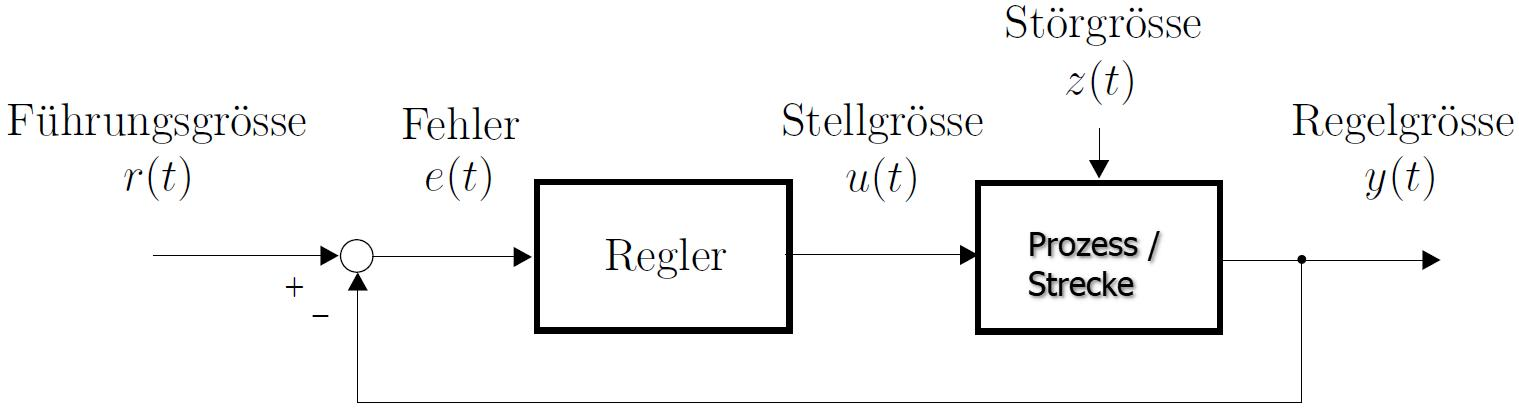
\includegraphics[width=0.85\columnwidth]{images/groessen_regelkreis.jpg}

	\vspace{0.2cm}

	\begin{tabular}{ l  l }
		\toprule
		Führungsgrösse $r(t)$ (Referenz)	& Gibt Sollwert vor 				\\
		\midrule
		Regelgrösse $y(t)$ 					& Zu regelnde Grösse 				\\
		\midrule
		Fehler $e(t)$ 						& Differenz $r(t) - y(t)$ 			\\
		\midrule
		Stellgrösse $u(t)$ 					& Regelerausgang / Streckeneingang	\\
		\midrule
		Störgrösse $z(t)$ (oder $d(t)$) 	& Störungen aller Art 				\\
		\bottomrule
	\end{tabular}
\end{center}


\subsection{Komponenten des Regelkreises}{16-17}

\begin{center}
	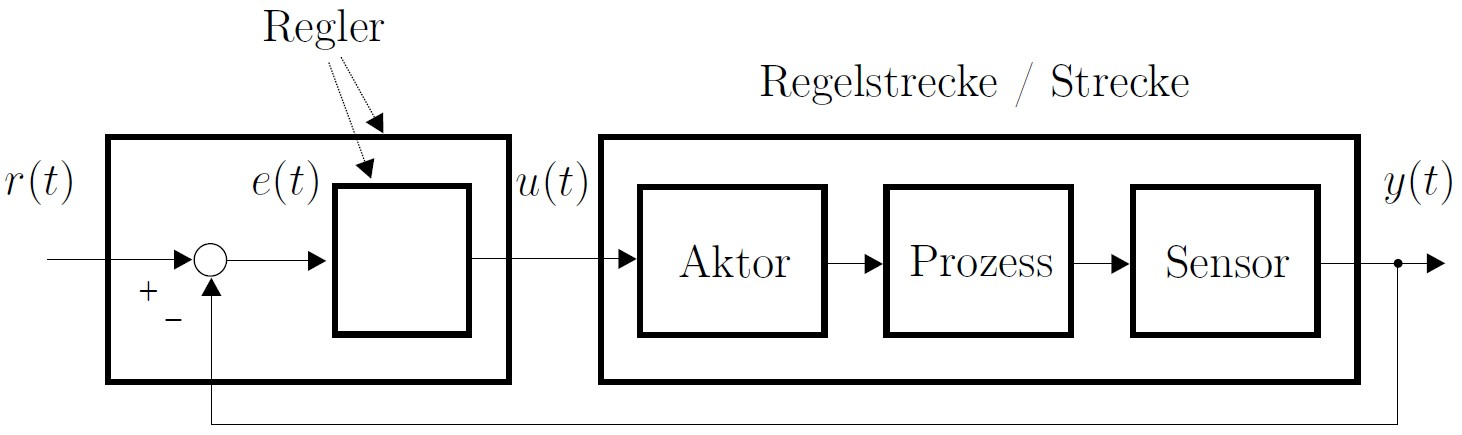
\includegraphics[width=0.8\columnwidth]{images/regler_regelstrecke.jpg}
\end{center}


\begin{itemize}
	\item \textbf{Genauigkeit beim Sensor wichtiger als beim Aktor!}
	\item Leistung liefert Aktor (Stellglied) 
\end{itemize}


\subsection{Steuerung vs. Regelung}{18-19}

Die Steuerungstechnik liefert oft die Führungsgrösse für geregelte Untersysteme.

\textbf{Eine Regelung hat Feedback bzgl. der Referenz, eine Steuerung nicht!}

\begin{center}
	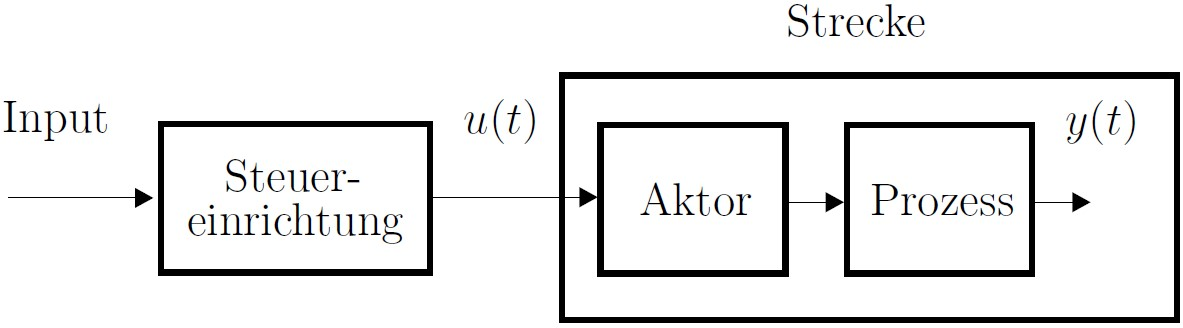
\includegraphics[width=0.8\columnwidth]{images/steuerung.jpg} 
\end{center}


\subsection{Prozess, System, Modell}{20}

\subsubsection{Prozess}
Gesamtheit zusammenwirkender Vorgänge, durch die Materie, Energie und Information umgeformt, transportiert und gespeichert wird.

\textrightarrow\ z.B. Fahren eines Autos (abstrakt)


\subsubsection{System}

Ist gegenüber der Umwelt abgegrenzt, hat Eingänge, Ausgänge (und Zustand).


\subsubsection{Modell}

Beschreibung von Systemen (häufig mit Hilfe der Mathematik)


\subsection{Modellierung}{21}

\begin{itemize}
	\item Ein Modell beschreibt \textbf{gewisse Aspekte} eines Prozesses
	\item Ein Modell beschreibt ein System \textbf{so genau wie nötig}
	\item \textbf{Alle Modelle sind falsch}
	\item Ein Modell muss an die Anwendung angepasst sein
\end{itemize}

\vspace{0.2cm}

Modellieren bedeutet, Systeme systematisch

\vspace{0.1cm}
\begin{itemize}
	\item in Teilsysteme zu teilen (Top-Down)
	\item aus Grundgliedern aufzubauen (Bottom-Up)
\end{itemize}

\columnbreak


\subsection{Beschreibungsmethoden von Systemen}

Alle genannten Methoden beschreiben ein System vollständig!

\vspace{0.2cm}

\begin{minipage}[t]{0.6\columnwidth}
	\raggedright

	\begin{itemize}
		\item Funktion oder LUT (statische Systeme)
		\item Sprungantwort (LZI-Systeme)
		\item Impulsantwort (auf Dirac-Stoss) 
		\item Übertragungsfunktion
		\item Frequenzgang
	\end{itemize}
\end{minipage}
\hfill
\begin{minipage}[t]{0.38\columnwidth}
	\raggedright

	\begin{itemize}
		\item Differenzialgleichungen
		\item Zustandsraum
		\item Block-Diagramm
		\item Bode-Diagramm
		\item Nyquist-Diagramm
		\item Pol-Nullstellen-Diagramm
	\end{itemize}
\end{minipage}

